\section{Auswertung}
\label{sec:Auswertung}
\subsection{Bestimmung der Zeitkonstanten RC}
Zur Bestimmung der Zeitkonstanten RC werden aus der Entladekurve in Abbildung \ref{fig:plotrc} die Werte für $U_\text{C}$ abgelesen.
$U_\text{0}$ wurde bestimmt zu $U_\text{0}=\SI{7.28}{\ohm}$.
Die abgelesenen Daten finden sich in Tabelle \ref{tab:taba}.
Durch Umformung wird Formel \eqref{eqn:aufladung} zu
\begin{equation}
	\label{eqn:ausgleich1}
	\ln\left(\frac{U_\text{C}}{U_\text{0}}\right)=-\frac{1}{RC}t .
\end{equation}
Zur Bestimmung der Zeitkonstanten $RC$ wird nun $\ln\left(\frac{U_\text{C}}{U_\text{0}}\right)$ gegen die Zeit $t$ aufgetragen.
Aus der Steigung der Regressionsgeraden nach Gleichung \eqref{eqn:ausgleich1} ergibt sich nun die berechnete Zeitkonstante zu

\begin{equation*}
	\centering
	RC = (0.48 \pm 0.03) \cdot 10^{-3} \si{\second} .
\end{equation*}
\begin{table}
	\caption{Messdaten zur Bestimmung der Zeitkonstanten $RC$}
	\label{tab:taba}
	\centering
	\begin{tabular}{ccc}
		\toprule
		$U_\text{C}$/$\si{\volt}$ & $\ln{(\frac{U_\text{C}}{U_\text{0}})}$ & $t$ /$10^{-3}\si{\second}$ \\
		\midrule
		6.04                      & -0.186726850262                        & 0.0                        \\
		4.04                      & -0.588886170236                        & 0.25                       \\
		2.76                      & -0.96990018248                         & 0.5                        \\
		1.8                       & -1.39734419731                         & 0.75                       \\
		1.08                      & -1.90816982107                         & 1.0                        \\
		0.56                      & -2.56494935746                         & 1.25                       \\
		0.24                      & -3.41224721785                         & 1.5                        \\
		\bottomrule
	\end{tabular}
\end{table}
Die Messdaten sowie die berechnete lineare Regression befinden sich in Abbildung \ref{fig:plota}.
\begin{figure}
	\centering
	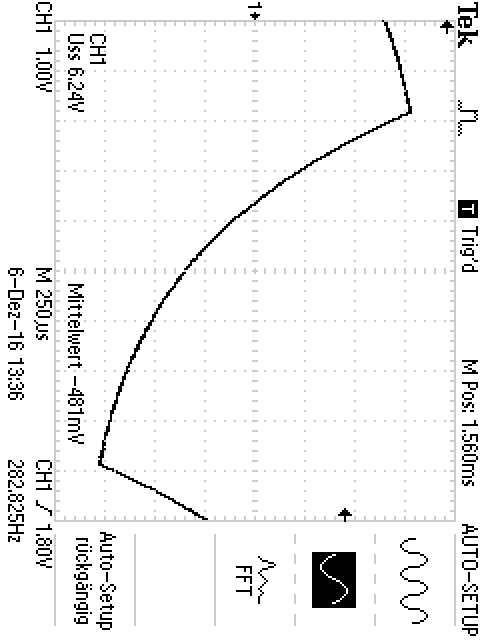
\includegraphics[angle=90]{bilder/F0000TEK.JPG}
	\caption{Aufgabenteil a: Entladekurve des Kondensators zur Bestimmung der Zeitkonstanten $RC$}
	\label{fig:plotrc}
\end{figure}

\begin{figure}
	\centering
	\includegraphics{build/test.pdf}
	\caption{Lineare Regression zur Bestimmung der Zeitkonstanten $RC$}
	\label{fig:plota}
\end{figure}

Die Zeitkonstante $RC$ soll nun erneut bestimmt werden, indem die Frequenzabhängigkeit der Amplitude $A(\omega)$ der Spannung $U_\text{C}$ am Kondensator untersucht wird.
Dazu wird $A(\omega)$ in Abhängigkeit zur Frequenz $\omega$ aufgetragen. Die verwendeten Daten befinden sich in Tabelle \ref{tab:tab2}.
Eine Regression mit Gleichung \eqref{eqn:amplitude} liefert für die Zeitkonstante :
\begin{equation*}
	\centering
	RC=(a = (RC) = 0.010 \pm 0.003)\cdot 10^{-3} \si{\second}
\end{equation*}

\begin{table}
	\caption{Messdaten zur Bestimmung der Zeitkonstanten $RC$ über die Frequenzabhängigkeit der Amplitude $A(\omega)$}
	\label{tab:tab2}
	\centering
	\begin{tabular}{cc}
		\toprule
		$A(\omega)$/ $10^{-3} \si{\volt}$ & $\omega$/$\si{\Hz}$ \\
		\midrule
		2800.0                            & 4.24                \\
		4400.0                            & 10.0                \\
		4880.0                            & 15.0                \\
		5040.0                            & 20.0                \\
		5200.0                            & 35.0                \\
		5120.0                            & 60.0                \\
		4880.0                            & 90.0                \\
		4320.0                            & 150.0               \\
		3600.0                            & 230.0               \\
		2880.0                            & 320.0               \\
		2080.0                            & 500.0               \\
		1120.0                            & 1000.0              \\
		680.0                             & 2000.0              \\
		230.0                             & 5000.0              \\
		120.0                             & 10000.0             \\
		\bottomrule
	\end{tabular}
\end{table}

Die Messdaten und die berechnete Regression sind in Abbildung \refeq{fig:plotb} abgebildet.
\begin{figure}
	\centering
	\includegraphics{build/amplitude.pdf}
	\caption{Regression zur Bestimmung der Zeitkonstanten $RC$ über die Frequenzabhängigkeit der Amplitude}
	\label{fig:plotb}
\end{figure}

\subsection{d) Integration}

\begin{figure}
	\centering
	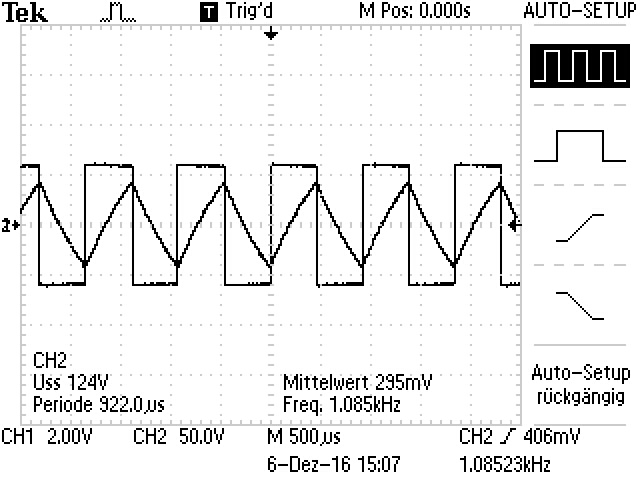
\includegraphics[width=0.75\textwidth]{bilder/ALL0001/F0001TEK.JPG}
	\caption{Aufgabenteil d: Rechteckspannung}
	\label{fig:rechteck}
\end{figure}

In Abbildung \ref{fig:rechteck} ist die Rechteckspannung sowie die über das RC-Glied integrierte Rechteckspannung dargestellt.
Die integrierte Rechteckspannung ist wie zu erwarten eine Dreiecksspannung.


\begin{figure}
	\centering
	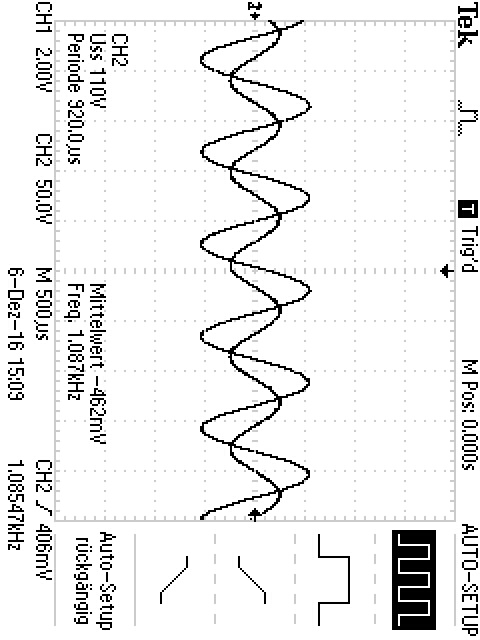
\includegraphics[width=0.75\textwidth]{bilder/ALL0002/F0002TEK.JPG}
	\caption{Aufgabenteil d: Sinusspannung}
	\label{fig:sinus}
\end{figure}

Der Spannungsverlauf der Sinusspannung ist in Abbildung \ref{fig:sinus} dargestellt. Wie zuvor ist die Kosinusspannung - integrierte Sinusspannung - außerdem in diesem Plot aufgezeichnet.


\begin{figure}
	\centering
	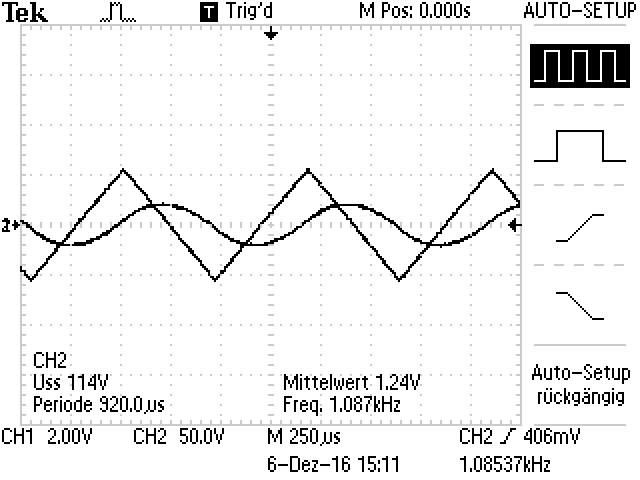
\includegraphics[width=0.75\textwidth]{bilder/ALL0003/F0003TEK.JPG}
	\caption{Aufgabenteil d: Dreiecksspannung}
	\label{fig:dreieck}
\end{figure}

In Abbildung \ref{fig:dreieck} ist Dreieck und Parabelspannung zu sehen
